\documentclass{standalone}
\usepackage{amsmath} % Required for \varPsi below
\usepackage{pgfplots}
\usepackage{tikz}
\usetikzlibrary{calc}
\usetikzlibrary{patterns}
\pgfplotsset{compat=1.14}


\newcommand*{\xMin}{0}%
\newcommand*{\xMax}{6}%
\newcommand*{\yMin}{0}%
\newcommand*{\yMax}{6}%

\begin{document}
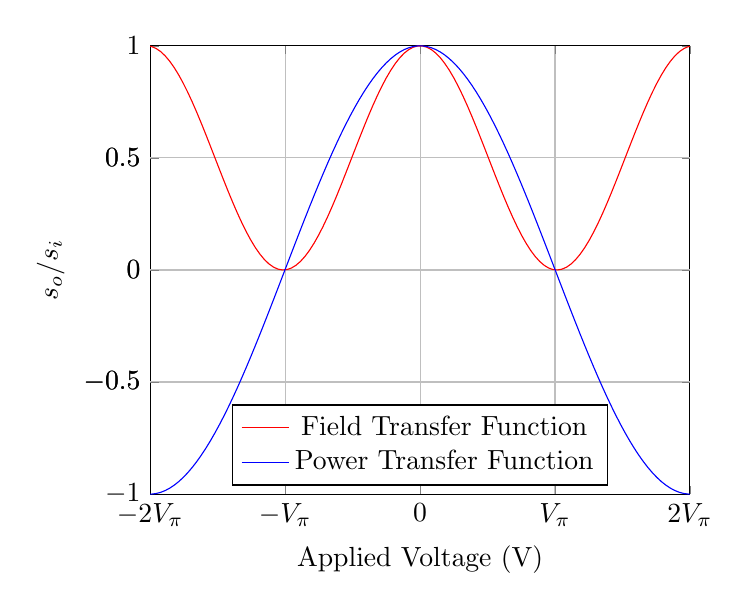
\begin{tikzpicture}
	\begin{axis}[
	xmin=-2,   xmax=2,
	ymin=-1,   ymax=1,
	%extra x ticks={-1,0,1},
	extra y ticks={-0.5,0,0.5},
	%extra tick style={grid=major, dashed},
	xtick={-2,-1,0,1,2}, 
	tick style={grid=major, dashed},
	xticklabels={$-2V_\pi$,$-V_\pi$,0,$V_\pi$,$2V_\pi$},
	legend style={at={(0.5,+0.2)},anchor=north},
	xlabel=Applied Voltage (V),ylabel=$s_o/s_i$,
]
    \addplot[color=red,samples=300] {((cos(deg(x)*1.55)*(cos(deg(x)*1.55)))}; 
    \addplot[color=blue,samples=300] {cos(deg(x)*sqrt(2.46))}; 
    \legend{Field Transfer Function,Power Transfer Function};
	
    \end{axis}
\end{tikzpicture}
\end{document}